\documentclass[12pt,a4paper]{article}
\usepackage{kotex}
\usepackage{graphicx}
\usepackage{hyperref}
\usepackage{indentfirst}
\usepackage{subcaption}
\usepackage{multirow}
\usepackage{flafter}
\usepackage{tikz}
\usetikzlibrary{arrows, intersections, decorations.markings, positioning, backgrounds}
\setlength{\parskip}{2mm}
\usepackage{amsmath}
\usepackage[top=3cm, bottom=2.54cm, left=2.54cm, right=2.54cm]{geometry}
\usepackage[yyyymmdd]{datetime}
\renewcommand{\dateseparator}{-}
\usepackage{array}
\newcolumntype{L}[1]{>{\raggedright\let\newline\\\arraybackslash\hspace{0pt}}m{#1}}
\newcolumntype{C}[1]{>{\centering\let\newline\\\arraybackslash\hspace{0pt}}m{#1}}
\newcolumntype{R}[1]{>{\raggedleft\let\newline\\\arraybackslash\hspace{0pt}}m{#1}}

\begin{document}
\begin{titlepage}
    \centering
    \begin{tabular}{|C{15cm}|}
        \hline
        \rule{0in}{6ex}
        {\huge 물리학 및 실험 1\par} \\ 
        {\large 스마트 게이트를 활용한 포사체 운동\par} \\
        \hline
    \end{tabular} \\
    \vspace{5cm}
    \includegraphics[height=7.36cm]{logo.png}\par
    \vspace{3cm}
    \begin{tabular}{|l|l|l|l|l|l|}
        \hline
        과목 & \multicolumn{5}{l|}{물리학및실험1} \\
        \hline
        담당교수 & \multicolumn{2}{l|}{전계진} & 담당조교 & \multicolumn{2}{l|}{} \\
        \hline
        조 및 조원 & \multicolumn{5}{l|}{2조, 김민수 김민규 김민서 김백준 김연주} \\
        \hline
        제출일 & \multicolumn{5}{l|}{\today} \\
        \hline
        작성자 & 김민수 & 학번 & 20518009 & 학과 & 정보보호 \\
        \hline
    \end{tabular}
\end{titlepage}
\section{실험목적}
포사체의 운동을 통해 중력 가속도를 받으면서 운동하는 물체의 2차원 운동을 이해한다.
포사체의 수평도달거리와 비행시간을 측정하여 이론적으로 유도된 값과 잘 들어맞는지 확인하고,
발사각에 따라 그 값이 또 어떻게 달라지는지 확인한다.
\section{실험원리}
포사체(projectile)는 초기 속도가 주어지고 이후에는 중력 가속도의 영향만으로 경로가 결정되는
물체이다 (실제로는 공기 저항도 포사체의 운동에 영향을 주지만, 이상적인 경우에는 이를 무시할 수 있다.)

Figure~\ref{fig1}과 같이 공을 수평방향에 대해 각 $\theta$, 초기속도 $v_{0}$로 발사하는 경우를 생각해보자.
Figure~\ref{fig1}의 점선은 포사체의 경로를 나타내는 곡선으로 포물선이 된다.

이 운동을 기술하기 위해 포사체가 $xy$평면상에서 운동한다고 가정하고, $x$축을 수평, $y$축을 위쪽
수직 방향으로 정하자. 이 포사체가 받는 가속도의 $x$성분은 $0$이고, $y$성분은 $-g$이다.
다시 말해, 포사체가 받는 가속도 $a$의 성분은 다음과 같다.
\begin{equation}
    a_{x} = 0, \quad\quad a_{y} = -g
\end{equation}
따라서 등가속도 운동식을 사용하여 다음과 같이 포사체의 속도와 위치를 구할 수 있다.
\begin{equation}
    \begin{aligned}
        &v_{x} = v_{0x} + a_{x}t=v_{0x} \\
        &v_{y} = v_{0y} + a_{y}t=v_{0y} - gt
        \label{eq2}
    \end{aligned}
\end{equation}
\begin{figure}[hbt!]
    \centering
    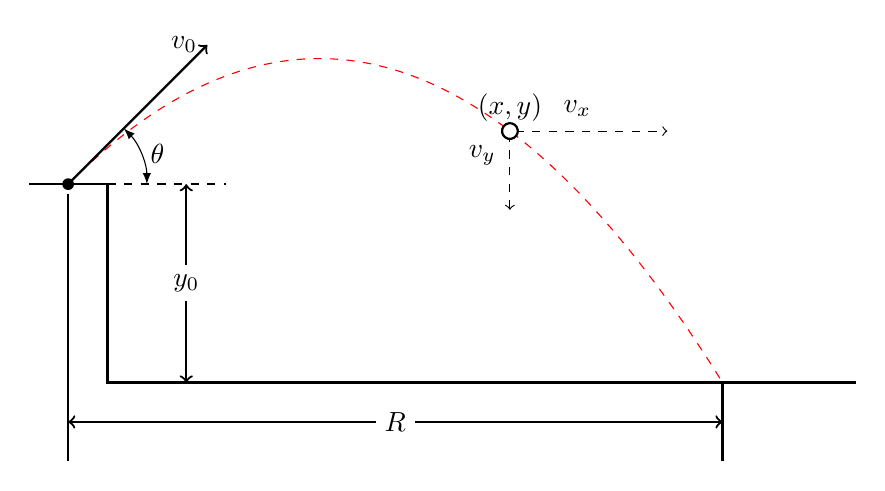
\begin{tikzpicture}[
            scale=10,
            tangent/.style={
                decoration={
                    markings,% switch on markings
                    mark=
                        at position #1
                        with
                        {
                            \coordinate (tangent point-\pgfkeysvalueof{/pgf/decoration/mark info/sequence number}) at (0pt,0pt);
                            \coordinate (tangent unit vector-\pgfkeysvalueof{/pgf/decoration/mark info/sequence number}) at (1,0pt);
                            \coordinate (tangent orthogonal unit vector-\pgfkeysvalueof{/pgf/decoration/mark info/sequence number}) at (0pt,1);
                        }
                },
                postaction=decorate
            },
            use tangent/.style={
                shift=(tangent point-#1),
                x=(tangent unit vector-#1),
                y=(tangent orthogonal unit vector-#1)
            },
            use tangent/.default=1
        ]
        \draw[-, thick] (-.05, 0.252) -- (.05, 0.252)  |- (1, 0);
        \draw[-, thick, dashed] (.05, 0.252) -- (0.2, 0.252);
        \draw[<->, thick] (0.15, 0.252) -- (0.15, 0) node at (0.15, 0.126)[fill=white] {$y_{0}$};
        \draw[-, thick] (0, 0.240) -- (0, -0.1);
        \node at (0, 0.252)[circle, fill=black, inner sep=1.5pt]{};

        \draw[red, tangent=0, tangent=0.6, name path=parabolaOne, domain=0:0.470155, samples=200, dashed, variable=\t]
            plot ({2.5 * cos(45) * \t}, {2.5 * sin(45) * \t - 9.8/2 * (\t)^2 + 0.252});

        \draw[-, thick] ({2.5 * cos(45) * 0.470155}, 0) -- ({2.5 * cos(45) * 0.470155}, -0.1);
        \draw[->, thick, use tangent] (0, 0) -- (2.5, 0) node at (2.5, 0) [left] {$v_{0}$};
        \draw[<->, thick] (0, -.05) -- ({2.5 * cos(45) * 0.470155}, -.05) node at ({2.5 * cos(45) * 0.470155 / 2}, -.05)[fill=white] {$R$};
        \filldraw[color=black!100, fill=white!100, thick, use tangent=2] (0, 0) circle(0.1);

        \node(nodeXY)[name path=nodeXY, circle, fill=white, inner sep=1.5pt, use tangent=2]{};

        \node at (0, 0)[use tangent=2, above]{$(x,y)$};
        \draw[latex-latex]  (0.1, 0.252) arc(0:45:0.1) node[midway,right]{$\theta$};
        % \node at [name path=nodeXY, circle, fill=white, inner sep=1.5pt, use tangent=2]{};
        \path[name intersections={of=parabolaOne and nodeXY, by=xyPos}];
        \node(belowPos)[below=1cm of nodeXY] at (nodeXY) {};
        \node(rightPos)[right=2cm of nodeXY] at (nodeXY) {};
        \begin{scope}[on background layer]
            \draw[<->, dashed, behind path] (belowPos) |- (rightPos);
        \end{scope}
        \node[below left=0cm of nodeXY] {$v_{y}$};
        \node[above right=0cm and 0.5cm of nodeXY] {$v_{x}$};
    \end{tikzpicture}
    \caption{\label{fig1} 포사체의 운동. 수평방향에 대해 각 $\theta$, 초기속도 $v_{0}$로 발사한 포사체는 포물선 궤적을 그리며 운동한다.}
\end{figure}
\begin{equation}
    \begin{aligned}
        & x = x_{0} + v_{0x}t + \frac{1}{2}a_{x}t^2 = x_{0} + v_{0x}t \\
        & y = y_{0} + v_{0y}t + \frac{1}{2}a_{y}t^2 = y_{0} + v_{0y}t - \frac{1}{2}gt^2
    \end{aligned}
\end{equation}

위 식으로부터 포사체의 운동은 수평방향($x$축)과 연직방향($y$축)을 두 축으로 하는 2차원 운동이 되고,
공기의 저항을 무시할 때 수평방향으로는 등속도 운동, 수평방향으로는 등가속도 운동으로 기술할 수 있다.

공을 발사하는 순간을 $t = 0$ 으로 설정하면, 초기속도 $v_{0} = (v_{0}cos\theta, v_{0}sin\theta)$가 되고,
$t$초 후의 공의 속도 $\vec{v} = (v_x, v_y)$는 식~\ref{eq2}로부터
\begin{equation}
    \begin{aligned}
        & v_x = v_0 cos\theta \\
        & v_y = v_0 sin\theta - gt
        \label{eq4}
    \end{aligned}
\end{equation}
가 된다.
\begin{figure}[hbt!]
    \centering
    \begin{subfigure}[b]{0.4\linewidth}
        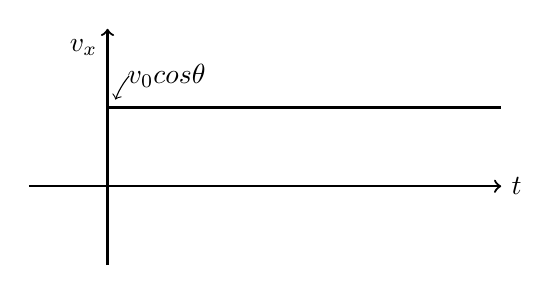
\begin{tikzpicture}
            \draw[->, thick] (-1,0) -- (5, 0) node(t)[right]{$t$};
            \draw[->, thick] (0,-1) -- (0, 2) node(v_x)[below left]{$v_x$};
            \draw[-, thick] (0, 1) node (point){} -- (5, 1);
            \node[above right=0cm of point] {$v_0cos\theta$};
            \draw[<-] (0.1,1.1) arc (-20:-40:-1);
        \end{tikzpicture}
    \end{subfigure}
    \begin{subfigure}[b]{0.4\linewidth}
        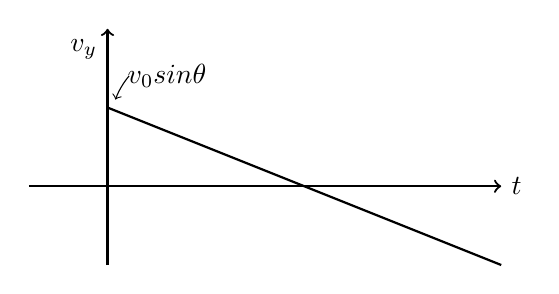
\begin{tikzpicture}
            \draw[->, thick] (-1,0) -- (5, 0) node(t)[right]{$t$};
            \draw[->, thick] (0,-1) -- (0, 2) node(v_y)[below left]{$v_y$};
            \draw[-, thick] (0, 1) node (point){} -- (5, -1);
            \node[above right=0cm of point] {$v_0sin\theta$};
            \draw[<-] (0.1,1.1) arc (-20:-40:-1);
        \end{tikzpicture}
    \end{subfigure}
    \caption{\label{fig2} 포사체의 속도. 시간에 따른 포사체의 속도 $v_x(t)$와 $v_y(t).$}
\end{figure}
또한 공이 발사되고 $t$초 후의 공의 위치 $(x, y)$는
\begin{equation}
    \begin{aligned}
        & x(t)=x_0 + (v_0 cos\theta)t \\
        & y(t)=y_0 + (v_0 sin\theta)t - \frac{1}{2}gt^2
        \label{eq5}
    \end{aligned}
\end{equation}
가 된다. 여기서 $x_0$와 $y_0$는 공이 발사될 때의 초기 위치$(x_0, y_0)$이다.
\begin{figure}[hbt!]
    \centering
    \begin{subfigure}[b]{0.4\linewidth}
        \begin{tikzpicture}
            \draw[->, thick] (-1,0) -- (5, 0) node(t)[right]{$t$};
            \draw[->, thick] (0,-1) -- (0, 2) node(x)[above]{$x$};
            \draw[-, thick] (0, 0.5) node (point){} -- (5, 2);
            \node[left=0cm of point] {$x_0$};
        \end{tikzpicture}
    \end{subfigure}
    \begin{subfigure}[b]{0.4\linewidth}
        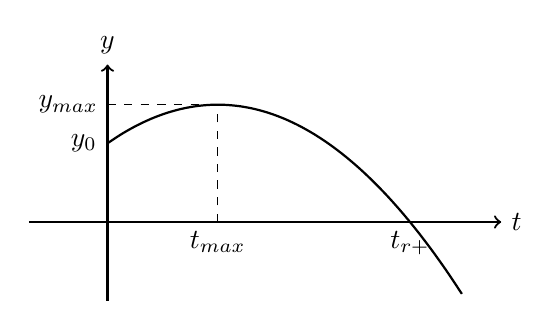
\begin{tikzpicture}
            \draw[->, thick] (-1,0) -- (5, 0) node(t)[right]{$t$};
            \draw[->, thick] (0,-1) -- (0, 2) node(x)[above]{$y$};
            \draw[-, thick, domain=0:4.5, smooth]
                plot(\x, {0.7 * \x - 0.25 * (\x)^2 + 1});
            \draw(-0.3, 1) node[] {$y_0$};
            \draw[-, dashed] (1.4,0) node[below]{$t_{max}$} -- (1.4, 1.49);
            \draw[-, dashed] (0,1.49) node[left]{$y_{max}$} -- (1.4, 1.49);
            \draw(3.84131, 0) node[below]{$t_{r+}$};
        \end{tikzpicture}
    \end{subfigure}
    \caption{\label{fig3} 포사체의 위치. 시간에 따른 포사체의 위치 $x(t)$와 $y(t)$.}
\end{figure}
\subsection{최고점 높이, $y_{max}$}
포사체가 최고 높이$(y_{max})$에 이르렀을 때, 수직방향의 속도, 즉 $v_y=0$이 된다. 만약 포사체가 최고 높이에 도달했을때의
시간을 $t_{max}$, 바닥으로부터의 높이를 $y_{max}$라고 하면, 식~\ref{eq4}의 두 번째 식에서
\begin{equation}
    \begin{aligned}
        & v_y=v_0 sin\theta - gt_{max} = 0
    \end{aligned}
\end{equation}
이 되고, 이 식으로부터 최고점 도달 시간 $t_{max}$는
\begin{equation}
    \begin{aligned}
        & t_{max}=\frac{v_0 sin\theta}{g}
    \end{aligned}
\end{equation}
이 된다. 이 값을 식~\ref{eq5}의 두 번째 식에 대입하면, 최고 높이 $y_{max}$는
\begin{equation}
    \begin{aligned}
        y_{max} &= y_0+(v_0 sin\theta)\frac{v_0 sin\theta}{g} - \frac{g}{2}\left(\frac{v_0 sin\theta}{g}\right)^2 \\
        &= y_0+\frac{v_0^2 sin^2\theta}{2g}
    \end{aligned}
\end{equation}
이 된다.
\subsection{수평 도달 거리, $R$}
다음에는 포사체가 바닥에 닿을 때까지 날아간 거리, 즉 포사체의 수평도달거리 $R$을 구하는 식을 유도해 보자

포사체가 바닥에 닿는 지점은 $(R, 0)$인 점이다. 만약 포사체가 바닥에 떨어질 때까지 날아간 시간을 $t_r$이라고 하면,
식~\ref{eq5}의 두 번째 식에서
\begin{equation}
    \begin{aligned}
        0=y_0+(v_0 sin\theta)t_r-\frac{1}{2}gt_r^2
    \end{aligned}
\end{equation}
을 만족한다. 따라서 $t_r$은 2차 방정식의 근의 공식을 이용하여
\begin{equation}
    \begin{aligned}
        t_{r\pm}=\frac{v_0 sin\theta\pm\sqrt{v_0^2 sin^2\theta+2gy_0}}{g}
        \label{eq10}
    \end{aligned}
\end{equation}
임을 알 수 있다. 여기서 우리가 구하는 답은 $t_{r+}$가 된다 $(t_{r+} > 0$ 이고 $t_{r-} < 0$인데, 음의 값은 공이 발사되기
 전 시간이므로 $t_{r+}$가 구하는 답이 된다). 수평도달거리 $R$은 $t_{r+}$를 식~\ref{eq5}의 첫 번째 
 식에 대입하여 다음과 같이 구할 수 있다.
 \begin{equation}
    \begin{aligned}
        R&=x_0+(v_0 cos\theta)t_{r+} \\
        &=x_0+(v_0 cos\theta)\frac{v_0 sin\theta+\sqrt{v_0^2 sin^2\theta+2gy_0}}{g}
        \label{eq11}
    \end{aligned}
\end{equation}
\subsection{포사체의 초기 속도, $v_0$}
이론적으로 포사체의 최고점 도달 높이와 수평도달거리를 알아내려면 포사체의 발사각 $\theta$와 초기위치$(x_0,y_0)$ 외에 포사체의
발사속도 $v_0$도 알아야 한다. $v_0$는 다음과 같은 방법으로 알아낼 수 있다.
\paragraph{[방법 1] 스마트 게이트를 이용하여 발사속도를 측정한다.}
\begin{flushleft}
포사체 발사 장치에 스마트 게이트를 장착하여 공이 발사되는 순간의 초기 속도$v_0$를 직접 측정할 수 있다.
이 실험에서는 이 방법을 사용할 것이다.
\end{flushleft}
\section{실험장치 및 방법}
스마트 게이트를 이용한 포사체 운동 실험에 필요한 실험 장치 및 기구는 다음과 같다.
\subsection{역학 실험장치}
    - 포사체 발사장치, 발사체(공), 테이블 클램프

    - 측량 추, 줄자, 종이, 먹지
\subsection{센서 실험장치}
    - 컴퓨터, PASCO 550 Interface, 데이터 분석 소프트웨어(Capstone)

    - 스마트 게이트(고정막대, 케이블, 고정 볼트 포함), Time of Flight
\subsection{실험 방법}
\subsubsection{실험 장치 구성}
\begin{enumerate}
    \item 책상 한쪽 끝에 발사 장치를 단단히 고정하고, 발사구에 연직추를 매달아서 수평 이동거리의 기준점을 표시한다.
    \item 550 인터페이스와 스마트 게이트를 연결한다.
    \item 발사강도를 1단(또는 2단)으로 하여 공을 장전하여 발사한다. 막대로 공을 발사구에 밀어 넣어서 공을 발사한 다음 공이
    날아가는 거리에 맞추어, 'Time of Flight' 장치를 갖다 놓고 스마트 게이트에 연결한다.
    \item 공이 바닥에 떨어지는 지점에 흰 종이를 고정시키고, 그 위를 먹지롤 덮어서 떨어진 지점이 종이 위에 표시되게 한다.
    \item 줄자를 이용하여 테이블에서 발사구까지 높이에서 Time of Flight 높이를 뺀 $y_0$를 측정한다.
\end{enumerate}
\subsubsection{센서와 캡스톤 프로그램 설정}
\begin{enumerate}
    \item 550 인터페이스의 스위치를 켠 후 Capstone 프로그램을 실행한다.
    \item 550 인터페이스가 정상적으로 인식되면, 좌측 [Tools]의 [Hardware Setup]을 클릭하면 다음 그림과 같이 화면에 550
    인터페이스가 나타난다.
    \item 550 인터페이스가 스마트 게이트를 인식하면, 다음과 같이 [Timer Setup]과 스마트게이트 아이콘이 나타난다.
    \item {[Hardware Setup]} 선택 후 Smart Gate 아이콘에서 3을 선택하여 Time of Flight Accessory를 선택한다.
    \item {[Timer Setup]}에서 Time of Flight 설정을 해준다. (전부 Next)
    \item {[Display]} 팔레트에서 [Table] 아이콘을 드래그하여 데이터 테이블을 생성한다. 오른쪽 [Display] 팔레트에서 [Table]
    을 화면 가운데로 드래그하면 테이블이 생성된다. Table에 1열은 Initial Speed(m/s)와 2열은 Time of Flight(s)를 선택한다.
\end{enumerate}
\subsubsection{본 실험}
실험 장치 구성과 센서 설정이 모두 끝났으면, 이제부터 포사체 운동 실험을 시작한다.
\begin{enumerate}
    \item {\label{enum2}발사구에 공을 넣고, 발사 강도를 1단으로 하여 장전한다.}
    \item {\label{enum1}발사각을 $15^{\circ}$로 고정하고 시험 발사하여 공이 떨어지는 위치를 확인한다.}
    \item 위 \ref{enum1}에서 확인한 위치에 Time of Flight 패드를 두고, 그 위에 흰 종이를 붙인 다음 먹지로 덮는다.
    \item 실험 준비가 완료되면, [Controls] 메뉴의 [Record] 버튼을 클릭한다. [Record] 버튼을 클릭하면 측정이 시작되고,
    [Record] 버튼은 [Stop] 버튼으로 바뀐다. 공을 발사하면 Initial Speed(m/s)와 2열은 Time of Filght(s)가 화면의
    표에 나타난다. 측정을 종료할 때에는 [Stop]을 클릭한다. 이때의 수평 이동거리(비행거리 $R$)를 줄자로 재어서 표에
    기록한다.
    \item 측정된 모든 데이터는 메모리에 저장된다. 저장된 데이터는 자동으로 이름이 부여되고 목록에 표시되여 그래프 또는
    테이블에서 언제든지 불러올 수 있다. 불필요한 데이터는 [Controls]메뉴의 [Delete Last Run] 및 하위메뉴에서 삭제할 수
    있다.
    \item {[Controls]} 메뉴의 [Stop] 버튼을 클릭하여 측정을 완료한다.
    \item {\label{enum3}공의 발사속도 $v$와 비행시간 $T$, 그리고 비행거리 $R$을 실험표에 기록한다.}
    \item {\label{enum4}위 \ref{enum2} $\sim$ \ref{enum3}의 과정을 3번 되풀이하고, 평균값과 표준오차를 기록한다.}
    \item 발사각을 $15^{\circ}$씩 증가시키면서 위 \ref{enum2} $\sim$ \ref{enum4}의 과정을 되풀이한다.
    \item 위의 결과로부터 발사각에 따른 도달거리의 변화를 보여주는 그래프를 그린다.
\end{enumerate}
\section{실험 결과 및 분석}
\begin{figure}[hbt!]
    \centering
    \begin{tikzpicture}[
            scale=10,
            tangent/.style={
                decoration={
                    markings,% switch on markings
                    mark=
                        at position #1
                        with
                        {
                            \coordinate (tangent point-\pgfkeysvalueof{/pgf/decoration/mark info/sequence number}) at (0pt,0pt);
                            \coordinate (tangent unit vector-\pgfkeysvalueof{/pgf/decoration/mark info/sequence number}) at (1,0pt);
                            \coordinate (tangent orthogonal unit vector-\pgfkeysvalueof{/pgf/decoration/mark info/sequence number}) at (0pt,1);
                        }
                },
                postaction=decorate
            },
            use tangent/.style={
                shift=(tangent point-#1),
                x=(tangent unit vector-#1),
                y=(tangent orthogonal unit vector-#1)
            },
            use tangent/.default=1
        ]
        \def\v{2.86}
        \def\deg{15}
        \def\rootAnsT{0.31456}
        \draw[-, thick] (-.05, 0.252) -- (.05, 0.252)  |- ({\v * cos(\deg) * \rootAnsT + 0.1}, 0);
        \draw[-, thick, dashed] (.05, 0.252) -- (0.2, 0.252);
        \draw[<->, thick] (0.15, 0.252) -- (0.15, 0) node at (0.15, 0.126)[fill=white, right] {$y_{0} = 0.2520m$};
        \draw[-, thick] (0, 0.240) -- (0, -0.1);
        \node at (0, 0.252)[circle, fill=black, inner sep=1.5pt]{};

        \draw[red, tangent=0, tangent=0.6, name path=parabolaOne, domain=0:\rootAnsT,
            samples=200, dashed, variable=\t]
            plot ({\v * cos(\deg) * \t}, {\v * sin(\deg) * \t - 9.8/2 * (\t)^2 + 0.2520});

        \draw[->, thick, use tangent] (0, 0) -- (2.5, 0) node at (2.5, 0) [right] {$v_{0} = $\v$m/s$};
        \draw[latex-latex]  (0.2, 0.252) arc(0:\deg:0.2) node[midway, below right]{$\theta = $\deg$^{\circ}$};

        \draw[-, thick] ({\v * cos(\deg) * \rootAnsT}, 0) -- ({\v * cos(\deg) * \rootAnsT}, -0.1);
        \draw[<->, thick] (0, -.05) -- ({\v * cos(\deg) * \rootAnsT}, -.05)
            node at ({\v * cos(\deg) * \rootAnsT / 2}, -.05)[fill=white, below] {측정값 $R = 0.9180m$};
    \end{tikzpicture}
    \caption{\label{fig4} $\theta = 15^{\circ}$일 때의 포사체의 운동.}
\end{figure}
\begin{figure}[hbt!]
    \centering
    \begin{tikzpicture}[
            scale=10,
            tangent/.style={
                decoration={
                    markings,% switch on markings
                    mark=
                        at position #1
                        with
                        {
                            \coordinate (tangent point-\pgfkeysvalueof{/pgf/decoration/mark info/sequence number}) at (0pt,0pt);
                            \coordinate (tangent unit vector-\pgfkeysvalueof{/pgf/decoration/mark info/sequence number}) at (1,0pt);
                            \coordinate (tangent orthogonal unit vector-\pgfkeysvalueof{/pgf/decoration/mark info/sequence number}) at (0pt,1);
                        }
                },
                postaction=decorate
            },
            use tangent/.style={
                shift=(tangent point-#1),
                x=(tangent unit vector-#1),
                y=(tangent orthogonal unit vector-#1)
            },
            use tangent/.default=1
        ]
        \def\v{2.99}
        \def\deg{30}
        \def\rootAnsT{0.425865}
        \draw[-, thick] (-.05, 0.252) -- (.05, 0.252)  |- ({\v * cos(\deg) * \rootAnsT + 0.1}, 0);
        \draw[-, thick, dashed] (.05, 0.252) -- (0.2, 0.252);
        \draw[<->, thick] (0.15, 0.252) -- (0.15, 0) node at (0.15, 0.126)[fill=white, right] {$y_{0} = 0.2520m$};
        \draw[-, thick] (0, 0.240) -- (0, -0.1);
        \node at (0, 0.252)[circle, fill=black, inner sep=1.5pt]{};

        \draw[red, tangent=0, tangent=0.6, name path=parabolaOne, domain=0:\rootAnsT,
            samples=200, dashed, variable=\t]
            plot ({\v * cos(\deg) * \t}, {\v * sin(\deg) * \t - 9.8/2 * (\t)^2 + 0.2520});

        \draw[->, thick, use tangent] (0, 0) -- (2.5, 0) node at (2.5, 0) [right] {$v_{0} = $\v$m/s$};
        \draw[latex-latex]  (0.2, 0.252) arc(0:\deg:0.2) node[midway, right]{$\theta = $\deg$^{\circ}$};

        \draw[-, thick] ({\v * cos(\deg) * \rootAnsT}, 0) -- ({\v * cos(\deg) * \rootAnsT}, -0.1);
        \draw[<->, thick] (0, -.05) -- ({\v * cos(\deg) * \rootAnsT}, -.05)
            node at ({\v * cos(\deg) * \rootAnsT / 2}, -.05)[fill=white, below] {측정값 $R = 1.119m$};
    \end{tikzpicture}
    \caption{\label{fig5} $\theta = 30^{\circ}$일 때의 포사체의 운동.}
\end{figure}
\begin{figure}[hbt!]
    \centering
    \begin{tikzpicture}[
            scale=10,
            tangent/.style={
                decoration={
                    markings,% switch on markings
                    mark=
                        at position #1
                        with
                        {
                            \coordinate (tangent point-\pgfkeysvalueof{/pgf/decoration/mark info/sequence number}) at (0pt,0pt);
                            \coordinate (tangent unit vector-\pgfkeysvalueof{/pgf/decoration/mark info/sequence number}) at (1,0pt);
                            \coordinate (tangent orthogonal unit vector-\pgfkeysvalueof{/pgf/decoration/mark info/sequence number}) at (0pt,1);
                        }
                },
                postaction=decorate
            },
            use tangent/.style={
                shift=(tangent point-#1),
                x=(tangent unit vector-#1),
                y=(tangent orthogonal unit vector-#1)
            },
            use tangent/.default=1
        ]
        \def\v{3.07}
        \def\deg{45}
        \def\rootAnsT{0.538523}
        \draw[-, thick] (-.05, 0.252) -- (.05, 0.252)  |- ({\v * cos(\deg) * \rootAnsT + 0.1}, 0);
        \draw[-, thick, dashed] (.05, 0.252) -- (0.2, 0.252);
        \draw[<->, thick] (0.15, 0.252) -- (0.15, 0) node at (0.15, 0.126)[fill=white, right] {$y_{0} = 0.2520m$};
        \draw[-, thick] (0, 0.240) -- (0, -0.1);
        \node at (0, 0.252)[circle, fill=black, inner sep=1.5pt]{};

        \draw[red, tangent=0, tangent=0.6, name path=parabolaOne, domain=0:\rootAnsT,
            samples=200, dashed, variable=\t]
            plot ({\v * cos(\deg) * \t}, {\v * sin(\deg) * \t - 9.8/2 * (\t)^2 + 0.2520});

        \draw[->, thick, use tangent] (0, 0) -- (2.5, 0) node at (2.5, 0) [right] {$v_{0} = $\v$m/s$};
        \draw[latex-latex]  (0.2, 0.252) arc(0:\deg:0.2) node[midway, right]{$\theta = $\deg$^{\circ}$};

        \draw[-, thick] ({\v * cos(\deg) * \rootAnsT}, 0) -- ({\v * cos(\deg) * \rootAnsT}, -0.1);
        \draw[<->, thick] (0, -.05) -- ({\v * cos(\deg) * \rootAnsT}, -.05)
            node at ({\v * cos(\deg) * \rootAnsT / 2}, -.05)[fill=white, below] {측정값 $R = 1.174m$};
    \end{tikzpicture}
    \caption{\label{fig6} $\theta = 45^{\circ}$일 때의 포사체의 운동.}
\end{figure}
\begin{figure}[hbt!]
    \centering
    \begin{tikzpicture}[
            scale=10,
            tangent/.style={
                decoration={
                    markings,% switch on markings
                    mark=
                        at position #1
                        with
                        {
                            \coordinate (tangent point-\pgfkeysvalueof{/pgf/decoration/mark info/sequence number}) at (0pt,0pt);
                            \coordinate (tangent unit vector-\pgfkeysvalueof{/pgf/decoration/mark info/sequence number}) at (1,0pt);
                            \coordinate (tangent orthogonal unit vector-\pgfkeysvalueof{/pgf/decoration/mark info/sequence number}) at (0pt,1);
                        }
                },
                postaction=decorate
            },
            use tangent/.style={
                shift=(tangent point-#1),
                x=(tangent unit vector-#1),
                y=(tangent orthogonal unit vector-#1)
            },
            use tangent/.default=1
        ]
        \def\v{3.15}
        \def\deg{60}
        \def\rootAnsT{0.637414}
        \draw[-, thick] (-.05, 0.252) -- (.05, 0.252)  |- ({\v * cos(\deg) * \rootAnsT + 0.1}, 0);
        \draw[-, thick, dashed] (.05, 0.252) -- (0.2, 0.252);
        \draw[<->, thick] (0.15, 0.252) -- (0.15, 0) node at (0.15, 0.126)[fill=white, right] {$y_{0} = 0.2520m$};
        \draw[-, thick] (0, 0.240) -- (0, -0.1);
        \node at (0, 0.252)[circle, fill=black, inner sep=1.5pt]{};

        \draw[red, tangent=0, tangent=0.6, name path=parabolaOne, domain=0:\rootAnsT,
            samples=200, dashed, variable=\t]
            plot ({\v * cos(\deg) * \t}, {\v * sin(\deg) * \t - 9.8/2 * (\t)^2 + 0.2520});

        \draw[->, thick, use tangent] (0, 0) -- (2.5, 0) node at (2.5, 0) [right] {$v_{0} = $\v$m/s$};
        \draw[latex-latex]  (0.2, 0.252) arc(0:\deg:0.2) node[midway, right]{$\theta = $\deg$^{\circ}$};

        \draw[-, thick] ({\v * cos(\deg) * \rootAnsT}, 0) -- ({\v * cos(\deg) * \rootAnsT}, -0.1);
        \draw[<->, thick] (0, -.05) -- ({\v * cos(\deg) * \rootAnsT}, -.05)
            node at ({\v * cos(\deg) * \rootAnsT / 2}, -.05)[fill=white, below] {측정값 $R = 0.9780m$};
    \end{tikzpicture}
    \caption{\label{fig7} $\theta = 60^{\circ}$일 때의 포사체의 운동.}
\end{figure}
\begin{figure}[hbt!]
    \centering
    \begin{tikzpicture}[
            scale=10,
            tangent/.style={
                decoration={
                    markings,% switch on markings
                    mark=
                        at position #1
                        with
                        {
                            \coordinate (tangent point-\pgfkeysvalueof{/pgf/decoration/mark info/sequence number}) at (0pt,0pt);
                            \coordinate (tangent unit vector-\pgfkeysvalueof{/pgf/decoration/mark info/sequence number}) at (1,0pt);
                            \coordinate (tangent orthogonal unit vector-\pgfkeysvalueof{/pgf/decoration/mark info/sequence number}) at (0pt,1);
                        }
                },
                postaction=decorate
            },
            use tangent/.style={
                shift=(tangent point-#1),
                x=(tangent unit vector-#1),
                y=(tangent orthogonal unit vector-#1)
            },
            use tangent/.default=1
        ]
        \def\v{3.07}
        \def\deg{45}
        \def\rootAnsT{0.538523}
        \draw[-, thick] (-.05, 0.252) -- (.05, 0.252)  |- ({\v * cos(\deg) * \rootAnsT + 0.1}, 0);
        \draw[-, thick, dashed] (.05, 0.252) -- (0.2, 0.252);
        \draw[<->, thick] (0.15, 0.252) -- (0.15, 0) node at (0.15, 0.126)[fill=white, right] {$y_{0} = 0.2520m$};
        \draw[-, thick] (0, 0.240) -- (0, -0.32);
        \node at (0, 0.252)[circle, fill=black, inner sep=1.5pt]{};

        \def\v{2.86}
        \def\deg{15}
        \def\rootAnsT{0.31456}
        \draw[red, tangent=0, tangent=0.6, name path=parabolaOne, domain=0:\rootAnsT,
            samples=200, dashed, variable=\t]
            plot ({\v * cos(\deg) * \t}, {\v * sin(\deg) * \t - 9.8/2 * (\t)^2 + 0.2520});
        \draw[->, thick, use tangent] (0, 0) -- (2.5, 0) node at (2.5, 0) [right] {$v_{0} = $\v$m/s$};

        \draw[-, thick] ({\v * cos(\deg) * \rootAnsT}, 0) -- ({\v * cos(\deg) * \rootAnsT}, -0.11);
        \draw[<->, thick] (0, -.05) -- ({\v * cos(\deg) * \rootAnsT}, -.05)
            node at ({\v * cos(\deg) * \rootAnsT / 2}, -.05)[fill=white, below]
            {$\theta = $\deg$^{\circ}$ 측정값 $R = 0.9180m$};

        \def\v{2.99}
        \def\deg{30}
        \def\rootAnsT{0.425865}
        \draw[green, tangent=0, tangent=0.6, name path=parabolaOne, domain=0:\rootAnsT,
            samples=200, dashed, variable=\t]
            plot ({\v * cos(\deg) * \t}, {\v * sin(\deg) * \t - 9.8/2 * (\t)^2 + 0.2520});
        \draw[->, thick, use tangent] (0, 0) -- (2.5, 0) node at (2.5, 0) [right] {$v_{0} = $\v$m/s$};

        \draw[-, thick] ({\v * cos(\deg) * \rootAnsT}, 0) -- ({\v * cos(\deg) * \rootAnsT}, -0.25);
        \draw[<->, thick] (0, -.19) -- ({\v * cos(\deg) * \rootAnsT}, -.19)
            node at ({\v * cos(\deg) * \rootAnsT / 2}, -.19)[fill=white, below]
            {$\theta = $\deg$^{\circ}$ 측정값 $R = 1.119m$};

        \def\v{3.07}
        \def\deg{45}
        \def\rootAnsT{0.538523}
        \draw[blue, tangent=0, tangent=0.6, name path=parabolaOne, domain=0:\rootAnsT,
            samples=200, dashed, variable=\t]
            plot ({\v * cos(\deg) * \t}, {\v * sin(\deg) * \t - 9.8/2 * (\t)^2 + 0.2520});
        \draw[->, thick, use tangent] (0, 0) -- (2.5, 0) node at (2.5, 0) [above right] {$v_{0} = $\v$m/s$};

        \draw[-, thick] ({\v * cos(\deg) * \rootAnsT}, 0) -- ({\v * cos(\deg) * \rootAnsT}, -0.32);
        \draw[<->, thick] (0, -.26) -- ({\v * cos(\deg) * \rootAnsT}, -.26)
            node at ({\v * cos(\deg) * \rootAnsT / 2}, -.26)[fill=white, below]
            {$\theta = $\deg$^{\circ}$ 측정값 $R = 1.174m$};

        \def\v{3.15}
        \def\deg{60}
        \def\rootAnsT{0.637414}
        \draw[purple, tangent=0, tangent=0.6, name path=parabolaOne, domain=0:\rootAnsT,
            samples=200, dashed, variable=\t]
            plot ({\v * cos(\deg) * \t}, {\v * sin(\deg) * \t - 9.8/2 * (\t)^2 + 0.2520});
        \draw[->, thick, use tangent] (0, 0) -- (2.5, 0) node at (2.5, 0) [above left] {$v_{0} = $\v$m/s$};

        \draw[-, thick] ({\v * cos(\deg) * \rootAnsT}, 0) -- ({\v * cos(\deg) * \rootAnsT}, -0.18);
        \draw[<->, thick] (0, -.12) -- ({\v * cos(\deg) * \rootAnsT}, -.12)
            node at ({\v * cos(\deg) * \rootAnsT / 2}, -.12)[fill=white, below]
            {$\theta = $\deg$^{\circ}$ 측정값 $R = 0.9780m$};
    \end{tikzpicture}
    \caption{\label{fig8}}
\end{figure}
\begin{figure}[hbt!]
    \centering
    \begin{tabular}{|c|c|c|c|c|c|c|}
        \hline
        발사각 $\theta$ & 측정값 & 1차 & 2차 & 3차 & 평균 & 표준오차 \\
        \hline
        \multirow{3}{*}{$15^{\circ}$} & 초기 속도 $v$ & 2.73 & 2.92 & 2.92 & 2.86 & 0.06\\
        \cline{2-7}
                                      & 비행 거리 $R$ & 0.9180 & 0.9200 & 0.9160 & 0.9180 & 0.0012\\
        \cline{2-7}
                                      & 비행 시간 $T$ & 0.31 & 0.32 & 0.32 & 0.32 & 0\\
        \hline
        \multirow{3}{*}{$30^{\circ}$} & 초기 속도 $v$ & 2.99 & 2.98 & 2.99 & 2.99 & 0\\
        \cline{2-7}
                                      & 비행 거리 $R$ & 1.115 & 1.113 & 1.129 & 1.119 & 0.0050\\
        \cline{2-7}
                                      & 비행 시간 $T$ & 0.42 & 0.42 & 0.43 & 0.42 & 0\\
        \hline
        \multirow{3}{*}{$45^{\circ}$} & 초기 속도 $v$ & 3.07 & 3.06 & 3.08 & 3.07 & 0.01\\
        \cline{2-7}
                                      & 비행 거리 $R$ & 1.178 & 1.174 & 1.170 & 1.174 & 0.0023\\
        \cline{2-7}
                                      & 비행 시간 $T$ & 0.53 & 0.53 & 0.53 & 0.53 & 0\\
        \hline
        \multirow{3}{*}{$60^{\circ}$} & 초기 속도 $v$ & 3.15 & 3.14 & 3.15 & 3.15 & 0\\
        \cline{2-7}
                                      & 비행 거리 $R$ & 0.9800 & 0.9820 & 0.9720 & 0.9780 & 0.0031\\
        \cline{2-7}
                                      & 비행 시간 $T$ & 0.63 & 0.64 & 0.63 & 0.63 & 0\\
        \hline
    \end{tabular}
    \caption{\label{fig9} 실험 결과 기록표.}
\end{figure}
이론값의 계산은 우선 비행 시간 $T$의 경우 식~\ref{eq10}에서 $t_{r+}$가 된다. $(t_{r+} > 0$ 이고 $t_{r-} < 0$인데, 음의 값은 공이 발사되기
전 시간이므로 $t_{r+}$가 구하는 답이 되기 때문.)

비행 거리 $R$은 식~\ref{eq10}에서 구한 값을 토대로 식~\ref{eq11}에서 구할 수 있다.
\begin{figure}[hbt!]
    \centering
    \begin{tabular}{|c|c|c|c|c|}
        \hline
        \multirow{2}{*}{$\theta$} & \multicolumn{2}{c|}{비행 시간 $T$ [s]} & \multicolumn{2}{c|}{비행 거리 $R$ [m]} \\
        \cline{2-5}
        & 이론치 & 상대 오차[\%] & 이론치 & 상대 오차[\%] \\
        \hline
        $15^{\circ}$ & 0.31 & 3 & 0.87 & 5.3 \\
        \hline
        $30^{\circ}$ & 0.43 & 2 & 1.10 & 1.5 \\
        \hline
        $45^{\circ}$ & 0.54 & 2 & 1.17 & 0.4 \\
        \hline
        $60^{\circ}$ & 0.64 & 2 & 1.00 & 2.7 \\
        \hline
    \end{tabular}
    \caption{\label{fig10} 이론값 계산 및 오차.}
\end{figure}
\section{실험 고찰}
    \subsection{고찰질문: 교수가 제시하는 문제에 답하기}
        \subsubsection{각도에 따른 비행시간 $t_r$와 비행거리 $R$를 그래프로 그려 보세요}
        Figure~\ref{fig11}, Figure~\ref{fig12} 참조.
        \begin{figure}[hbt!]
            \centering
            \begin{tikzpicture}[
                    scale=10,
                    tangent/.style={
                        decoration={
                            markings,% switch on markings
                            mark=
                                at position #1
                                with
                                {
                                    \coordinate (tangent point-\pgfkeysvalueof{/pgf/decoration/mark info/sequence number}) at (0pt,0pt);
                                    \coordinate (tangent unit vector-\pgfkeysvalueof{/pgf/decoration/mark info/sequence number}) at (1,0pt);
                                    \coordinate (tangent orthogonal unit vector-\pgfkeysvalueof{/pgf/decoration/mark info/sequence number}) at (0pt,1);
                                }
                        },
                        postaction=decorate
                    },
                    use tangent/.style={
                        shift=(tangent point-#1),
                        x=(tangent unit vector-#1),
                        y=(tangent orthogonal unit vector-#1)
                    },
                    use tangent/.default=1
                ]
                \def\v{3.07}
                \def\deg{45}
                \def\rootAnsT{0.538523}
                \draw[-, thick] (-.05, 0.252) -- (.05, 0.252)  |- ({\rootAnsT + 0.1}, 0);
                \draw[-, thick, dashed] (.05, 0.252) -- (0.2, 0.252);
                \draw[<->, thick] (0.15, 0.252) -- (0.15, 0) node at (0.15, 0.126)[fill=white, right] {$y_{0} = 0.2520m$};
                \draw[-, thick] (0, 0.240) -- (0, -0.32);
                \node at (0, 0.252)[circle, fill=black, inner sep=1.5pt]{};
        
                \def\v{2.86}
                \def\deg{15}
                \def\rootAnsT{0.31456}
                \draw[red, tangent=0, tangent=0.6, name path=parabolaOne, domain=0:\rootAnsT,
                    samples=200, dashed]
                    plot (\x, {\v * sin(\deg) * \x - 9.8/2 * (\x)^2 + 0.2520});
                \draw[->, thick, use tangent] (0, 0) -- (2.5, 0) node at (2.5, 0) [right] {$v_{0} = $\v$m/s$};
        
                \draw[-, thick] (\rootAnsT, 0) -- (\rootAnsT, -0.11);
                \draw[<->, thick] (0, -.05) -- (\rootAnsT, -.05)
                    node at ({\rootAnsT / 2}, -.05)[fill=white, below]
                    {$\theta = $\deg$^{\circ}$ 측정값 $t_r = $0.32$s$};
        
                \def\v{2.99}
                \def\deg{30}
                \def\rootAnsT{0.425865}
                \draw[green, tangent=0, tangent=0.6, name path=parabolaOne, domain=0:\rootAnsT,
                    samples=200, dashed]
                    plot (\x, {\v * sin(\deg) * \x - 9.8/2 * (\x)^2 + 0.2520});
                \draw[->, thick, use tangent] (0, 0) -- (2.5, 0) node at (2.5, 0) [right] {$v_{0} = $\v$m/s$};
        
                \draw[-, thick] (\rootAnsT, 0) -- (\rootAnsT, -0.18);
                \draw[<->, thick] (0, -.12) -- (\rootAnsT, -.12)
                    node at ({\rootAnsT / 2}, -.12)[fill=white, below]
                    {$\theta = $\deg$^{\circ}$ 측정값 $t_r = $0.42$s$};
        
                \def\v{3.07}
                \def\deg{45}
                \def\rootAnsT{0.538523}
                \draw[blue, tangent=0, tangent=0.6, name path=parabolaOne, domain=0:\rootAnsT,
                    samples=200, dashed]
                    plot (\x, {\v * sin(\deg) * \x - 9.8/2 * (\x)^2 + 0.2520});
                \draw[->, thick, use tangent] (0, 0) -- (2.5, 0) node at (2.5, 0) [above right] {$v_{0} = $\v$m/s$};
        
                \draw[-, thick] (\rootAnsT, 0) -- (\rootAnsT, -0.25);
                \draw[<->, thick] (0, -.19) -- (\rootAnsT, -.19)
                    node at ({\rootAnsT / 2}, -.19)[fill=white, below]
                    {$\theta = $\deg$^{\circ}$ 측정값 $t_r = $0.53$s$};
        
                \def\v{3.15}
                \def\deg{60}
                \def\rootAnsT{0.637414}
                \draw[purple, tangent=0, tangent=0.6, name path=parabolaOne, domain=0:\rootAnsT,
                    samples=200, dashed]
                    plot (\x, {\v * sin(\deg) * \x - 9.8/2 * (\x)^2 + 0.2520});
                \draw[->, thick, use tangent] (0, 0) -- (2.5, 0) node at (2.5, 0) [above left] {$v_{0} = $\v$m/s$};
        
                \draw[-, thick] (\rootAnsT, 0) -- (\rootAnsT, -0.32);
                \draw[<->, thick] (0, -.26) -- (\rootAnsT, -.26)
                    node at ({\rootAnsT / 2}, -.26)[fill=white, below]
                    {$\theta = $\deg$^{\circ}$ 측정값 $t_r = $0.63$s$};
            \end{tikzpicture}
            \caption{\label{fig11}}
        \end{figure}
        \begin{figure}[hbt!]
            \centering
            \begin{tikzpicture}[
                    scale=10,
                    tangent/.style={
                        decoration={
                            markings,% switch on markings
                            mark=
                                at position #1
                                with
                                {
                                    \coordinate (tangent point-\pgfkeysvalueof{/pgf/decoration/mark info/sequence number}) at (0pt,0pt);
                                    \coordinate (tangent unit vector-\pgfkeysvalueof{/pgf/decoration/mark info/sequence number}) at (1,0pt);
                                    \coordinate (tangent orthogonal unit vector-\pgfkeysvalueof{/pgf/decoration/mark info/sequence number}) at (0pt,1);
                                }
                        },
                        postaction=decorate
                    },
                    use tangent/.style={
                        shift=(tangent point-#1),
                        x=(tangent unit vector-#1),
                        y=(tangent orthogonal unit vector-#1)
                    },
                    use tangent/.default=1
                ]
                \def\v{3.07}
                \def\deg{45}
                \def\rootAnsT{0.538523}
                \draw[-, thick] (-.05, 0.252) -- (.05, 0.252)  |- ({\v * cos(\deg) * \rootAnsT + 0.1}, 0);
                \draw[-, thick, dashed] (.05, 0.252) -- (0.2, 0.252);
                \draw[<->, thick] (0.15, 0.252) -- (0.15, 0) node at (0.15, 0.126)[fill=white, right] {$y_{0} = 0.2520m$};
                \draw[-, thick] (0, 0.240) -- (0, -0.32);
                \node at (0, 0.252)[circle, fill=black, inner sep=1.5pt]{};
        
                \def\v{2.86}
                \def\deg{15}
                \def\rootAnsT{0.31456}
                \draw[red, tangent=0, tangent=0.6, name path=parabolaOne, domain=0:\rootAnsT,
                    samples=200, dashed, variable=\t]
                    plot ({\v * cos(\deg) * \t}, {\v * sin(\deg) * \t - 9.8/2 * (\t)^2 + 0.2520});
                \draw[->, thick, use tangent] (0, 0) -- (2.5, 0) node at (2.5, 0) [right] {$v_{0} = $\v$m/s$};
        
                \draw[-, thick] ({\v * cos(\deg) * \rootAnsT}, 0) -- ({\v * cos(\deg) * \rootAnsT}, -0.11);
                \draw[<->, thick] (0, -.05) -- ({\v * cos(\deg) * \rootAnsT}, -.05)
                    node at ({\v * cos(\deg) * \rootAnsT / 2}, -.05)[fill=white, below]
                    {$\theta = $\deg$^{\circ}$ 측정값 $R = 0.9180m$};
        
                \def\v{2.99}
                \def\deg{30}
                \def\rootAnsT{0.425865}
                \draw[green, tangent=0, tangent=0.6, name path=parabolaOne, domain=0:\rootAnsT,
                    samples=200, dashed, variable=\t]
                    plot ({\v * cos(\deg) * \t}, {\v * sin(\deg) * \t - 9.8/2 * (\t)^2 + 0.2520});
                \draw[->, thick, use tangent] (0, 0) -- (2.5, 0) node at (2.5, 0) [right] {$v_{0} = $\v$m/s$};
        
                \draw[-, thick] ({\v * cos(\deg) * \rootAnsT}, 0) -- ({\v * cos(\deg) * \rootAnsT}, -0.25);
                \draw[<->, thick] (0, -.19) -- ({\v * cos(\deg) * \rootAnsT}, -.19)
                    node at ({\v * cos(\deg) * \rootAnsT / 2}, -.19)[fill=white, below]
                    {$\theta = $\deg$^{\circ}$ 측정값 $R = 1.119m$};
        
                \def\v{3.07}
                \def\deg{45}
                \def\rootAnsT{0.538523}
                \draw[blue, tangent=0, tangent=0.6, name path=parabolaOne, domain=0:\rootAnsT,
                    samples=200, dashed, variable=\t]
                    plot ({\v * cos(\deg) * \t}, {\v * sin(\deg) * \t - 9.8/2 * (\t)^2 + 0.2520});
                \draw[->, thick, use tangent] (0, 0) -- (2.5, 0) node at (2.5, 0) [above right] {$v_{0} = $\v$m/s$};
        
                \draw[-, thick] ({\v * cos(\deg) * \rootAnsT}, 0) -- ({\v * cos(\deg) * \rootAnsT}, -0.32);
                \draw[<->, thick] (0, -.26) -- ({\v * cos(\deg) * \rootAnsT}, -.26)
                    node at ({\v * cos(\deg) * \rootAnsT / 2}, -.26)[fill=white, below]
                    {$\theta = $\deg$^{\circ}$ 측정값 $R = 1.174m$};
        
                \def\v{3.15}
                \def\deg{60}
                \def\rootAnsT{0.637414}
                \draw[purple, tangent=0, tangent=0.6, name path=parabolaOne, domain=0:\rootAnsT,
                    samples=200, dashed, variable=\t]
                    plot ({\v * cos(\deg) * \t}, {\v * sin(\deg) * \t - 9.8/2 * (\t)^2 + 0.2520});
                \draw[->, thick, use tangent] (0, 0) -- (2.5, 0) node at (2.5, 0) [above left] {$v_{0} = $\v$m/s$};
        
                \draw[-, thick] ({\v * cos(\deg) * \rootAnsT}, 0) -- ({\v * cos(\deg) * \rootAnsT}, -0.18);
                \draw[<->, thick] (0, -.12) -- ({\v * cos(\deg) * \rootAnsT}, -.12)
                    node at ({\v * cos(\deg) * \rootAnsT / 2}, -.12)[fill=white, below]
                    {$\theta = $\deg$^{\circ}$ 측정값 $R = 0.9780m$};
            \end{tikzpicture}
            \caption{\label{fig12}}
        \end{figure}
        \subsubsection{발사각이 $30^{\circ}$인 경우와 $60^{\circ}$인 경우의 도달거리가 같은가? 다르다면 다른 이유는
        무엇인가?}
        Figure~\ref{fig12}를 보면 $\theta$가 $30^\circ$일 때와 $60^\circ$일 때의 도달 거리는 다른데,
        그 이유는 포사체의 발사 위치가 원점이 아닌 $(0, y_0)$위치에 있기 때문이다.
        \begin{figure}[hbt!]
            \centering
            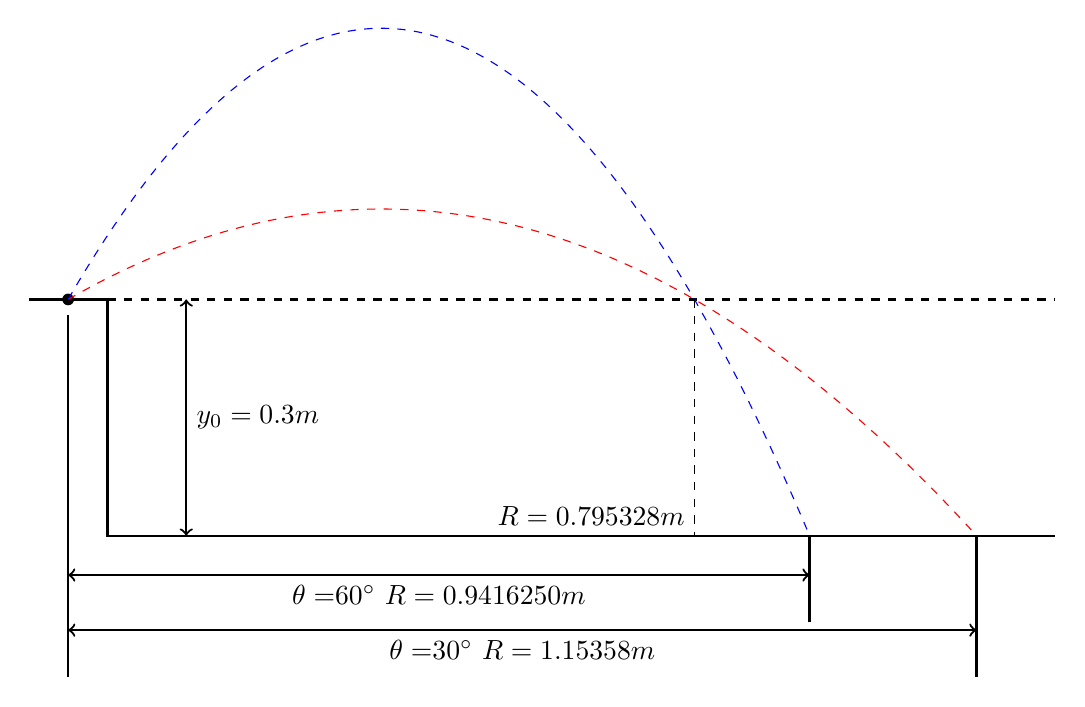
\begin{tikzpicture}[scale=10]
                \def\v{3}
                \def\deg{30}
                \def\rootAnsT{0.444012}
                \draw[-, thick] (-.05, 0.3) -- (.05, 0.3)  |- ({\v * cos(\deg) * \rootAnsT + 0.1}, 0);
                \draw[-, thick, dashed] (.05, 0.3) -- ({\v * cos(\deg) * \rootAnsT + 0.1}, 0.3);
                \draw[<->, thick] (0.15, 0.3) -- (0.15, 0) node at (0.15, 0.15)[fill=white, right] {$y_{0} = 0.3m$};
                \draw[-, thick] (0, 0.28) -- (0, -0.18);
                \node at (0, 0.3)[circle, fill=black, inner sep=1.5pt]{};
        
                
                \def\deg{30}
                \def\rootAnsT{0.444012}
                \draw[red, name path=parabolaOne, domain=0:\rootAnsT, samples=200, dashed, variable=\t]
                    plot ({\v * cos(\deg) * \t}, {\v * sin(\deg) * \t - 9.8/2 * (\t)^2 + 0.3});
        
                \draw[-, thick] ({\v * cos(\deg) * \rootAnsT}, 0) -- ({\v * cos(\deg) * \rootAnsT}, -0.18);
                \draw[<->, thick] (0, -.12) -- ({\v * cos(\deg) * \rootAnsT}, -.12)
                    node at ({\v * cos(\deg) * \rootAnsT / 2}, -.12)[fill=white, below]
                    {$\theta = $\deg$^{\circ}$ $R = 1.15358m$};
        
                \def\deg{60}
                \def\rootAnsT{0.62775}
                \draw[blue, name path=parabolaOne, domain=0:\rootAnsT, samples=200, dashed, variable=\t]
                    plot ({\v * cos(\deg) * \t}, {\v * sin(\deg) * \t - 9.8/2 * (\t)^2 + 0.3});
        
                \draw[-, thick] ({\v * cos(\deg) * \rootAnsT}, 0) -- ({\v * cos(\deg) * \rootAnsT}, -0.11);
                \draw[<->, thick] (0, -.05) -- ({\v * cos(\deg) * \rootAnsT}, -.05)
                    node at ({\v * cos(\deg) * \rootAnsT / 2}, -.05)[fill=white, below]
                    {$\theta = $\deg$^{\circ}$ $R = 0.9416250m$};

                \draw[dashed] (0.795328, 0.3) -- (0.795328, 0)
                    node[fill=white, above left] {$R = 0.795328m$};
            \end{tikzpicture}
            \caption{\label{fig13}}
        \end{figure}
        Figure~\ref{fig13}을 보면 더 확실해지는데, $y_0=0$이고 공기저항이 없는 환경에서의 포사체는
        $\theta$가 $30^\circ$와 $60^\circ$인 두 포사체는, 같은 지점에 도달한다.
        그러나 $y_0=0.3m$와 같이 주어지면 $\theta$가 $30^\circ$와 $60^\circ$인 두 포사체는 도달거리가 차이가 나는 것을
        알 수 있다.
        \subsubsection{도달거리가 최대인 발사각은 얼마인가?(이것은 초기 발사 높이에 따라 달라지는지 살펴보세요)}
        Figure~\ref{fig12}에 따르면, 도달거리가 제일 먼 발사각은 $\theta=45^{\circ}$일 때이며, 이것은 초기 발사각에
        따라 차차 도달거리가 증가하다가 $\theta=45^{\circ}$ 이후의 $\theta=60^{\circ}$인 포사체에선
        오히려 도달거리가 줄어드는 것을 확인할 수 있다.
    \subsection{오차원인:}
    실험 측정결과 표~\ref{fig9}를 보면 $\theta=15^{\circ}$인 포사체의 측정결과가 특히 부정확한 것을 알 수 있는데,
    $\theta=15^{\circ}$인 포사체를 측정할 때에 포사체 발사장치를 고정하는 클램프의 힘이 약하여 발사장치가 살짝 움직였던
    것이 원인이 아닐까 한다. 또한 모든 데이터의 상대 오차가 $\theta=15^{\circ}$인 포사체의 측정 데이터를 제외하고
    1\%$\sim$3\%정도의 상대 오차를 보이고 있는데, 이는 아마도 공기의 저항이 아닌가 한다. 통상적으로는 공기 저항에 의해
    더 가까운 곳까지 도달했어야 할 $\theta=15^{\circ}$인 포사체가 오히려 먼 곳까지 도달한 것은 단순 측정 실수로 보여진다.
    이러한 오차원인을 제거하기 위해선, 클램프를 꽉 조이고 되도록 조작에 과도한 힘을 사용하지 않도록 하여 포사체 발사장치의
    움직임을 줄여야 할 것이다.
    \subsection{실험을 통해 배우게 된 것}
    \begin{itemize}
        \item 초기 속도$v_0$와 $\theta$가 주어지면 해당 포사체의 도달 거리와 시간을 구하는 법을 배웠다.
        \item 스마트 게이트와 Time of Flight장비의 사용법을 배웠다.
        \item 포사체의 투사각도$\theta$가 $\theta=45^{\circ}$일때 무조건 제일 멀리 도달하진 않는다는 사실을 배웠다.
        \item [etc..]
    \end{itemize}
    \subsection{실험원리의 실생활에서의 예}
    \begin{enumerate}
    \item 총기의 탄도학이나 대륙간 탄도미사일의 탄도계산
    \item 인공위성의 안정적인 궤도 유지를 위한 계산
    \item 게임 안의 물리엔진의 동작 원리
    \item [etc..]
    \end{enumerate}
\end{document}